\section{Apache Cordova}

Apache Cordova, o Cordova a secas, se trata de un entorno de desarrollo de aplicaciones móviles utilizando tecnologías web, \gls{HTML} y \gls{CSS} para la presentación, \emph{JavaScript} para la lógica. Es posible que hayas escuchado hablar sobre algo llamado \emph{PhoneGap}, pues bien, antes de continuar, convendría explicar que relación existe entre ambos. Si nos remontamos a 2008, una empresa llamada \emph{Nitobi} presenta PhoneGap, un entorno para la creación de aplicaciones móviles usando tecnologías web (de momento no hay diferencias con Cordova). En 2011 deciden donar el código a la fundación \emph{Apache}, lo que supone que se convierta en software libre, y debido al éxito que tiene, ese mismo año, \emph{Adobe} compra \emph{Nitobi}, quedándose con sus empleados, sus proyectos, sus marcas, \ldots y dentro de este paquete se encuentra PhoneGap. Decide entonces mantener PhoneGap como software Open Source, pero debido a que la marca PhoneGap pertenece a \emph{Adobe}, optan por cambiarle el nombre, surgiendo así Apache Cordova\footnote{\url{https://www.campusmvp.es/recursos/post/PhoneGap-o-Apache-Cordova-que-diferencia-hay.aspx}}. Así que como vemos, ambos proyectos se tratan del mismo. La única diferencia destacable es el servicio \emph{Adobe PhoneGap Build}\footnote{\url{https://build.phonegap.com/}}, que nos permite compilar nuestro código en la nube a cualquier plataforma sin necesidad de tener que tener instalado en nuestro ordenador la SDK de cada plataforma. Entonces, ¿Cuál debemos usar?. Cualquiera de los dos, al final, se trata de lo mismo. Lo único a tener en cuenta es si vamos a usar alguno de los servicios que ofrece Adobe.

Tras esta breve explicación, necesaria ya que siempre surge la duda, veamos como funciona Cordova. El objetivo es conseguir que nuestro código realizado con tecnologías web sea ejecutado en cualquier plataforma como si de una aplicación nativa se tratase. Para conseguir esto, Cordova proporciona un entorno nativo para cada plataforma sobre el cual, se ejecutará nuestra aplicación. Esta envoltura está compuesta por un navegador (WebView) que se encarga de ejecutar nuestro código, y si son necesario, una serie de plugins que permiten la comunicación entre nuestro código y las \glspl{API} de cada plataforma a través de una \gls{API} unificada. Estos plugins pueden ser ofrecidos por el propio Cordova, como ser realizados por terceros.

\begin{figure}[H]
\centering
  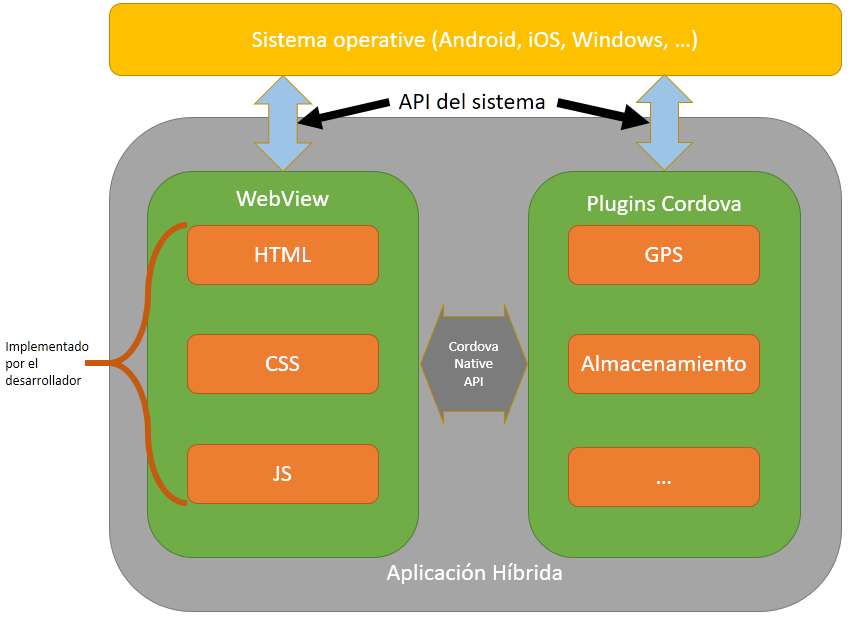
\includegraphics[width=0.8\textwidth]{Figures/ch1/cordova/diagram}
  \caption{Este diagrama muestra de forma simplificada como está compuesta una aplicación hibrida que utiliza Apache Cordova.}
\end{figure}

Cordova cuenta con una interfaz de línea de comandos (\gls{CLI}) con la podremos crear proyectos, compilarlos, ejecutarlos, \ldots. También nos servirá para añadir plugin a nuestro proyecto. El único requisito será el tener instalado en la máquina el SDK de las plataformas a las que vaya destinada nuestra aplicación.

Apache Cordova se encuentra disponible como paquete de \gls{npm}, desde donde puede ser instalada. Ver el anexo sobre \nameref{ch:ionic}.

Algunos de los frameworks que se utilizan para crear aplicaciones híbridas se colocan por ``encima'' de Cordova. Este es el caso de Ionic, framework en el que se centra este \gls{PFC}. Muchos de los comandos disponibles en Ionic \gls{CLI} no son más que envoltorios sobre el \gls{CLI} de Cordova, así como también ocurre con Ionic Native, que se coloca sobre los plugin de Cordova.
